\documentclass[1p]{elsarticle_modified}
%\bibliographystyle{elsarticle-num}

%\usepackage[colorlinks]{hyperref}
%\usepackage{abbrmath_seonhwa} %\Abb, \Ascr, \Acal ,\Abf, \Afrak
\usepackage{amsfonts}
\usepackage{amssymb}
\usepackage{amsmath}
\usepackage{amsthm}
\usepackage{scalefnt}
\usepackage{amsbsy}
\usepackage{kotex}
\usepackage{caption}
\usepackage{subfig}
\usepackage{color}
\usepackage{graphicx}
\usepackage{xcolor} %% white, black, red, green, blue, cyan, magenta, yellow
\usepackage{float}
\usepackage{setspace}
\usepackage{hyperref}

\usepackage{tikz}
\usetikzlibrary{arrows}

\usepackage{multirow}
\usepackage{array} % fixed length table
\usepackage{hhline}

%%%%%%%%%%%%%%%%%%%%%
\makeatletter
\renewcommand*\env@matrix[1][\arraystretch]{%
	\edef\arraystretch{#1}%
	\hskip -\arraycolsep
	\let\@ifnextchar\new@ifnextchar
	\array{*\c@MaxMatrixCols c}}
\makeatother %https://tex.stackexchange.com/questions/14071/how-can-i-increase-the-line-spacing-in-a-matrix
%%%%%%%%%%%%%%%

\usepackage[normalem]{ulem}

\newcommand{\msout}[1]{\ifmmode\text{\sout{\ensuremath{#1}}}\else\sout{#1}\fi}
%SOURCE: \msout is \stkout macro in https://tex.stackexchange.com/questions/20609/strikeout-in-math-mode

\newcommand{\cancel}[1]{
	\ifmmode
	{\color{red}\msout{#1}}
	\else
	{\color{red}\sout{#1}}
	\fi
}

\newcommand{\add}[1]{
	{\color{blue}\uwave{#1}}
}

\newcommand{\replace}[2]{
	\ifmmode
	{\color{red}\msout{#1}}{\color{blue}\uwave{#2}}
	\else
	{\color{red}\sout{#1}}{\color{blue}\uwave{#2}}
	\fi
}

\newcommand{\Sol}{\mathcal{S}} %segment
\newcommand{\D}{D} %diagram
\newcommand{\A}{\mathcal{A}} %arc


%%%%%%%%%%%%%%%%%%%%%%%%%%%%%5 test

\def\sl{\operatorname{\textup{SL}}(2,\Cbb)}
\def\psl{\operatorname{\textup{PSL}}(2,\Cbb)}
\def\quan{\mkern 1mu \triangleright \mkern 1mu}

\theoremstyle{definition}
\newtheorem{thm}{Theorem}[section]
\newtheorem{prop}[thm]{Proposition}
\newtheorem{lem}[thm]{Lemma}
\newtheorem{ques}[thm]{Question}
\newtheorem{cor}[thm]{Corollary}
\newtheorem{defn}[thm]{Definition}
\newtheorem{exam}[thm]{Example}
\newtheorem{rmk}[thm]{Remark}
\newtheorem{alg}[thm]{Algorithm}

\newcommand{\I}{\sqrt{-1}}
\begin{document}

%\begin{frontmatter}
%
%\title{Boundary parabolic representations of knots up to 8 crossings}
%
%%% Group authors per affiliation:
%\author{Yunhi Cho} 
%\address{Department of Mathematics, University of Seoul, Seoul, Korea}
%\ead{yhcho@uos.ac.kr}
%
%
%\author{Seonhwa Kim} %\fnref{s_kim}}
%\address{Center for Geometry and Physics, Institute for Basic Science, Pohang, 37673, Korea}
%\ead{ryeona17@ibs.re.kr}
%
%\author{Hyuk Kim}
%\address{Department of Mathematical Sciences, Seoul National University, Seoul 08826, Korea}
%\ead{hyukkim@snu.ac.kr}
%
%\author{Seokbeom Yoon}
%\address{Department of Mathematical Sciences, Seoul National University, Seoul, 08826,  Korea}
%\ead{sbyoon15@snu.ac.kr}
%
%\begin{abstract}
%We find all boundary parabolic representation of knots up to 8 crossings.
%
%\end{abstract}
%\begin{keyword}
%    \MSC[2010] 57M25 
%\end{keyword}
%
%\end{frontmatter}

%\linenumbers
%\tableofcontents
%
\newcommand\colored[1]{\textcolor{white}{\rule[-0.35ex]{0.8em}{1.4ex}}\kern-0.8em\color{red} #1}%
%\newcommand\colored[1]{\textcolor{white}{ #1}\kern-2.17ex	\textcolor{white}{ #1}\kern-1.81ex	\textcolor{white}{ #1}\kern-2.15ex\color{red}#1	}

{\Large $\underline{11n_{114}~(K11n_{114})}$}

\setlength{\tabcolsep}{10pt}
\renewcommand{\arraystretch}{1.6}
\vspace{1cm}\begin{tabular}{m{100pt}>{\centering\arraybackslash}m{274pt}}
\multirow{5}{120pt}{
	\centering
	\includegraphics[width=112pt]{../../../GIT/diagram.site/Diagrams/png/730_11n_114.png}\\
\ \ \ A knot diagram\footnotemark}&
\allowdisplaybreaks
\textbf{Linearized knot diagam} \\
\cline{2-2}
 &
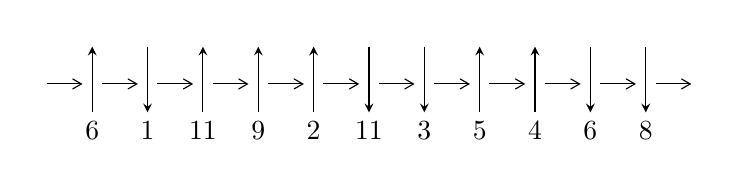
\begin{tikzpicture}[x=20pt, y=17pt]
	% nodes
	\node (C0) at (0, 0) {};
	\node (C1) at (1, 0) {};
	\node (C1U) at (1, +1) {};
	\node (C1D) at (1, -1) {6};

	\node (C2) at (2, 0) {};
	\node (C2U) at (2, +1) {};
	\node (C2D) at (2, -1) {1};

	\node (C3) at (3, 0) {};
	\node (C3U) at (3, +1) {};
	\node (C3D) at (3, -1) {11};

	\node (C4) at (4, 0) {};
	\node (C4U) at (4, +1) {};
	\node (C4D) at (4, -1) {9};

	\node (C5) at (5, 0) {};
	\node (C5U) at (5, +1) {};
	\node (C5D) at (5, -1) {2};

	\node (C6) at (6, 0) {};
	\node (C6U) at (6, +1) {};
	\node (C6D) at (6, -1) {11};

	\node (C7) at (7, 0) {};
	\node (C7U) at (7, +1) {};
	\node (C7D) at (7, -1) {3};

	\node (C8) at (8, 0) {};
	\node (C8U) at (8, +1) {};
	\node (C8D) at (8, -1) {5};

	\node (C9) at (9, 0) {};
	\node (C9U) at (9, +1) {};
	\node (C9D) at (9, -1) {4};

	\node (C10) at (10, 0) {};
	\node (C10U) at (10, +1) {};
	\node (C10D) at (10, -1) {6};

	\node (C11) at (11, 0) {};
	\node (C11U) at (11, +1) {};
	\node (C11D) at (11, -1) {8};
	\node (C12) at (12, 0) {};

	% arrows
	\draw[->,>={angle 60}]
	(C0) edge (C1) (C1) edge (C2) (C2) edge (C3) (C3) edge (C4) (C4) edge (C5) (C5) edge (C6) (C6) edge (C7) (C7) edge (C8) (C8) edge (C9) (C9) edge (C10) (C10) edge (C11) (C11) edge (C12) ;	\draw[->,>=stealth]
	(C1D) edge (C1U) (C2U) edge (C2D) (C3D) edge (C3U) (C4D) edge (C4U) (C5D) edge (C5U) (C6U) edge (C6D) (C7U) edge (C7D) (C8D) edge (C8U) (C9D) edge (C9U) (C10U) edge (C10D) (C11U) edge (C11D) ;
	\end{tikzpicture} \\
\hhline{~~} \\& 
\textbf{Solving Sequence} \\ \cline{2-2} 
 &
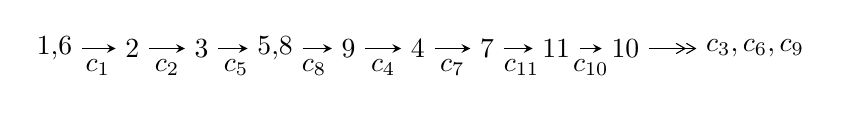
\begin{tikzpicture}[x=25pt, y=7pt]
	% node
	\node (A0) at (-1/8, 0) {1,6};
	\node (A1) at (1, 0) {2};
	\node (A2) at (2, 0) {3};
	\node (A3) at (49/16, 0) {5,8};
	\node (A4) at (33/8, 0) {9};
	\node (A5) at (41/8, 0) {4};
	\node (A6) at (49/8, 0) {7};
	\node (A7) at (57/8, 0) {11};
	\node (A8) at (65/8, 0) {10};
	\node (C1) at (1/2, -1) {$c_{1}$};
	\node (C2) at (3/2, -1) {$c_{2}$};
	\node (C3) at (5/2, -1) {$c_{5}$};
	\node (C4) at (29/8, -1) {$c_{8}$};
	\node (C5) at (37/8, -1) {$c_{4}$};
	\node (C6) at (45/8, -1) {$c_{7}$};
	\node (C7) at (53/8, -1) {$c_{11}$};
	\node (C8) at (61/8, -1) {$c_{10}$};
	\node (A9) at (10, 0) {$c_{3},c_{6},c_{9}$};

	% edge
	\draw[->,>=stealth]	
	(A0) edge (A1) (A1) edge (A2) (A2) edge (A3) (A3) edge (A4) (A4) edge (A5) (A5) edge (A6) (A6) edge (A7) (A7) edge (A8) ;
	\draw[->>,>={angle 60}]	
	(A8) edge (A9);
\end{tikzpicture} \\ 

\end{tabular} \\

\footnotetext{
The image of knot diagram is generated by the software ``\textbf{Draw programme}" developed by Andrew Bartholomew(\url{http://www.layer8.co.uk/maths/draw/index.htm\#Running-draw}), where we modified some parts for our purpose(\url{https://github.com/CATsTAILs/LinksPainter}).
}\phantom \\ \newline 
\centering \textbf{Ideals for irreducible components\footnotemark of $X_{\text{par}}$} 
 
\begin{align*}
I^u_{1}&=\langle 
-8.11096\times10^{17} u^{33}+9.35587\times10^{20} u^{32}+\cdots+6.89890\times10^{21} b+2.59045\times10^{22},\\
\phantom{I^u_{1}}&\phantom{= \langle  }2.18041\times10^{22} u^{33}+5.62075\times10^{22} u^{32}+\cdots+7.58879\times10^{22} a+3.69144\times10^{23},\;u^{34}+2 u^{33}+\cdots+7 u+11\rangle \\
I^u_{2}&=\langle 
u^6- u^5+2 u^4+3 u^2+b- u+1,\;3 u^7-3 u^6+8 u^5-2 u^4+12 u^3-2 u^2+a+7 u+1,\\
\phantom{I^u_{2}}&\phantom{= \langle  }u^8- u^7+3 u^6- u^5+5 u^4- u^3+4 u^2+1\rangle \\
\\
\end{align*}
\raggedright * 2 irreducible components of $\dim_{\mathbb{C}}=0$, with total 42 representations.\\
\footnotetext{All coefficients of polynomials are rational numbers. But the coefficients are sometimes approximated in decimal forms when there is not enough margin.}
\newpage
\renewcommand{\arraystretch}{1}
\centering \section*{I. $I^u_{1}= \langle -8.11\times10^{17} u^{33}+9.36\times10^{20} u^{32}+\cdots+6.90\times10^{21} b+2.59\times10^{22},\;2.18\times10^{22} u^{33}+5.62\times10^{22} u^{32}+\cdots+7.59\times10^{22} a+3.69\times10^{23},\;u^{34}+2 u^{33}+\cdots+7 u+11 \rangle$}
\flushleft \textbf{(i) Arc colorings}\\
\begin{tabular}{m{7pt} m{180pt} m{7pt} m{180pt} }
\flushright $a_{1}=$&$\begin{pmatrix}1\\0\end{pmatrix}$ \\
\flushright $a_{6}=$&$\begin{pmatrix}0\\u\end{pmatrix}$ \\
\flushright $a_{2}=$&$\begin{pmatrix}1\\- u^2\end{pmatrix}$ \\
\flushright $a_{3}=$&$\begin{pmatrix}u^2+1\\- u^2\end{pmatrix}$ \\
\flushright $a_{5}=$&$\begin{pmatrix}- u\\u^3+u\end{pmatrix}$ \\
\flushright $a_{8}=$&$\begin{pmatrix}-0.287320 u^{33}-0.740665 u^{32}+\cdots-3.53964 u-4.86434\\0.000117569 u^{33}-0.135614 u^{32}+\cdots+0.865413 u-3.75488\end{pmatrix}$ \\
\flushright $a_{9}=$&$\begin{pmatrix}0.143106 u^{33}+0.249396 u^{32}+\cdots-0.223580 u+1.42586\\0.104883 u^{33}-0.445287 u^{32}+\cdots+3.18850 u-8.62377\end{pmatrix}$ \\
\flushright $a_{4}=$&$\begin{pmatrix}0.0394778 u^{33}+0.431456 u^{32}+\cdots+0.666334 u+6.41410\\0.165129 u^{33}+0.482550 u^{32}+\cdots-3.55890 u+3.74557\end{pmatrix}$ \\
\flushright $a_{7}=$&$\begin{pmatrix}0.0368522 u^{33}-0.145447 u^{32}+\cdots+0.442048 u-2.59348\\0.0284463 u^{33}-0.271749 u^{32}+\cdots+3.02149 u-6.45999\end{pmatrix}$ \\
\flushright $a_{11}=$&$\begin{pmatrix}-0.707206 u^{33}-0.981033 u^{32}+\cdots-12.7294 u+3.24526\\0.738525 u^{33}+0.935117 u^{32}+\cdots+13.8701 u+0.827585\end{pmatrix}$ \\
\flushright $a_{10}=$&$\begin{pmatrix}-0.707206 u^{33}-0.981033 u^{32}+\cdots-12.7294 u+3.24526\\0.524915 u^{33}+0.603994 u^{32}+\cdots+9.12444 u+5.59476\end{pmatrix}$\\ \flushright $a_{10}=$&$\begin{pmatrix}-0.707206 u^{33}-0.981033 u^{32}+\cdots-12.7294 u+3.24526\\0.524915 u^{33}+0.603994 u^{32}+\cdots+9.12444 u+5.59476\end{pmatrix}$\\&\end{tabular}
\flushleft \textbf{(ii) Obstruction class $= -1$}\\~\\
\flushleft \textbf{(iii) Cusp Shapes $= \frac{7834694531803698284505}{6898902254749248769081} u^{33}+\frac{21981428947083072934378}{6898902254749248769081} u^{32}+\cdots+\frac{249772794381385562667795}{6898902254749248769081} u+\frac{89566862339158532678079}{6898902254749248769081}$}\\~\\
\newpage\renewcommand{\arraystretch}{1}
\flushleft \textbf{(iv) u-Polynomials at the component}\newline \\
\begin{tabular}{m{50pt}|m{274pt}}
Crossings & \hspace{64pt}u-Polynomials at each crossing \\
\hline $$\begin{aligned}c_{1},c_{5}\end{aligned}$$&$\begin{aligned}
&u^{34}-2 u^{33}+\cdots-7 u+11
\end{aligned}$\\
\hline $$\begin{aligned}c_{2}\end{aligned}$$&$\begin{aligned}
&u^{34}+14 u^{33}+\cdots+1117 u+121
\end{aligned}$\\
\hline $$\begin{aligned}c_{3}\end{aligned}$$&$\begin{aligned}
&u^{34}+5 u^{33}+\cdots+685 u+79
\end{aligned}$\\
\hline $$\begin{aligned}c_{4},c_{8},c_{9}\end{aligned}$$&$\begin{aligned}
&u^{34}- u^{33}+\cdots+11 u+7
\end{aligned}$\\
\hline $$\begin{aligned}c_{6},c_{10}\end{aligned}$$&$\begin{aligned}
&u^{34}+17 u^{32}+\cdots-235 u+25
\end{aligned}$\\
\hline $$\begin{aligned}c_{7}\end{aligned}$$&$\begin{aligned}
&u^{34}- u^{33}+\cdots+12 u+1
\end{aligned}$\\
\hline $$\begin{aligned}c_{11}\end{aligned}$$&$\begin{aligned}
&u^{34}+3 u^{33}+\cdots+13 u^2+1
\end{aligned}$\\
\hline
\end{tabular}\\~\\
\newpage\renewcommand{\arraystretch}{1}
\flushleft \textbf{(v) Riley Polynomials at the component}\newline \\
\begin{tabular}{m{50pt}|m{274pt}}
Crossings & \hspace{64pt}Riley Polynomials at each crossing \\
\hline $$\begin{aligned}c_{1},c_{5}\end{aligned}$$&$\begin{aligned}
&y^{34}+14 y^{33}+\cdots+1117 y+121
\end{aligned}$\\
\hline $$\begin{aligned}c_{2}\end{aligned}$$&$\begin{aligned}
&y^{34}+26 y^{33}+\cdots+5145 y+14641
\end{aligned}$\\
\hline $$\begin{aligned}c_{3}\end{aligned}$$&$\begin{aligned}
&y^{34}-39 y^{33}+\cdots-92711 y+6241
\end{aligned}$\\
\hline $$\begin{aligned}c_{4},c_{8},c_{9}\end{aligned}$$&$\begin{aligned}
&y^{34}+27 y^{33}+\cdots+75 y+49
\end{aligned}$\\
\hline $$\begin{aligned}c_{6},c_{10}\end{aligned}$$&$\begin{aligned}
&y^{34}+34 y^{33}+\cdots-2025 y+625
\end{aligned}$\\
\hline $$\begin{aligned}c_{7}\end{aligned}$$&$\begin{aligned}
&y^{34}+37 y^{33}+\cdots+238 y+1
\end{aligned}$\\
\hline $$\begin{aligned}c_{11}\end{aligned}$$&$\begin{aligned}
&y^{34}-5 y^{33}+\cdots+26 y+1
\end{aligned}$\\
\hline
\end{tabular}\\~\\
\newpage\flushleft \textbf{(vi) Complex Volumes and Cusp Shapes}
$$\begin{array}{c|c|c}  
\text{Solutions to }I^u_{1}& \I (\text{vol} + \sqrt{-1}CS) & \text{Cusp shape}\\
 \hline 
\begin{aligned}
u &= -0.644176 + 0.829926 I \\
a &= \phantom{-}1.09773 - 1.30377 I \\
b &= \phantom{-}1.18905 + 0.84583 I\end{aligned}
 & \phantom{-}3.62421 - 0.66236 I & \phantom{-}0.88799 + 2.20410 I \\ \hline\begin{aligned}
u &= -0.644176 - 0.829926 I \\
a &= \phantom{-}1.09773 + 1.30377 I \\
b &= \phantom{-}1.18905 - 0.84583 I\end{aligned}
 & \phantom{-}3.62421 + 0.66236 I & \phantom{-}0.88799 - 2.20410 I \\ \hline\begin{aligned}
u &= -0.634571 + 0.890410 I \\
a &= -0.522236 + 0.565118 I \\
b &= \phantom{-}0.98473 - 1.34431 I\end{aligned}
 & \phantom{-}3.43204 - 4.32834 I & \phantom{-}0.57903 + 4.14192 I \\ \hline\begin{aligned}
u &= -0.634571 - 0.890410 I \\
a &= -0.522236 - 0.565118 I \\
b &= \phantom{-}0.98473 + 1.34431 I\end{aligned}
 & \phantom{-}3.43204 + 4.32834 I & \phantom{-}0.57903 - 4.14192 I \\ \hline\begin{aligned}
u &= -0.287047 + 0.823608 I \\
a &= -0.04962 - 1.84400 I \\
b &= -0.090832 + 1.169670 I\end{aligned}
 & \phantom{-}1.321200 + 0.457071 I & -0.716277 + 1.122784 I \\ \hline\begin{aligned}
u &= -0.287047 - 0.823608 I \\
a &= -0.04962 + 1.84400 I \\
b &= -0.090832 - 1.169670 I\end{aligned}
 & \phantom{-}1.321200 - 0.457071 I & -0.716277 - 1.122784 I \\ \hline\begin{aligned}
u &= -0.483483 + 1.040970 I \\
a &= -0.808214 + 0.762258 I \\
b &= -0.602539 - 0.491415 I\end{aligned}
 & -0.58958 - 3.12068 I & \phantom{-}3.68668 + 4.96612 I \\ \hline\begin{aligned}
u &= -0.483483 - 1.040970 I \\
a &= -0.808214 - 0.762258 I \\
b &= -0.602539 + 0.491415 I\end{aligned}
 & -0.58958 + 3.12068 I & \phantom{-}3.68668 - 4.96612 I \\ \hline\begin{aligned}
u &= \phantom{-}0.895269 + 0.721333 I \\
a &= \phantom{-}0.693708 + 0.565955 I \\
b &= -0.88397 - 1.15926 I\end{aligned}
 & \phantom{-}8.26845 - 0.87317 I & \phantom{-}4.37441 - 0.26243 I \\ \hline\begin{aligned}
u &= \phantom{-}0.895269 - 0.721333 I \\
a &= \phantom{-}0.693708 - 0.565955 I \\
b &= -0.88397 + 1.15926 I\end{aligned}
 & \phantom{-}8.26845 + 0.87317 I & \phantom{-}4.37441 + 0.26243 I\\
 \hline 
 \end{array}$$\newpage$$\begin{array}{c|c|c}  
\text{Solutions to }I^u_{1}& \I (\text{vol} + \sqrt{-1}CS) & \text{Cusp shape}\\
 \hline 
\begin{aligned}
u &= \phantom{-}0.053846 + 0.825704 I \\
a &= -0.916529 + 0.670441 I \\
b &= -1.58656 - 0.18494 I\end{aligned}
 & -8.96690 + 0.23437 I & -4.99367 + 1.27444 I \\ \hline\begin{aligned}
u &= \phantom{-}0.053846 - 0.825704 I \\
a &= -0.916529 - 0.670441 I \\
b &= -1.58656 + 0.18494 I\end{aligned}
 & -8.96690 - 0.23437 I & -4.99367 - 1.27444 I \\ \hline\begin{aligned}
u &= -0.150608 + 0.812616 I \\
a &= -1.42827 - 1.83208 I \\
b &= -0.098454 - 0.251948 I\end{aligned}
 & \phantom{-}1.20998 - 2.44183 I & -2.48690 + 6.55623 I \\ \hline\begin{aligned}
u &= -0.150608 - 0.812616 I \\
a &= -1.42827 + 1.83208 I \\
b &= -0.098454 + 0.251948 I\end{aligned}
 & \phantom{-}1.20998 + 2.44183 I & -2.48690 - 6.55623 I \\ \hline\begin{aligned}
u &= \phantom{-}0.448396 + 0.692842 I \\
a &= \phantom{-}0.180015 + 1.383330 I \\
b &= \phantom{-}0.984901 - 0.373416 I\end{aligned}
 & -1.69966 + 1.41305 I & -2.63563 + 1.93957 I \\ \hline\begin{aligned}
u &= \phantom{-}0.448396 - 0.692842 I \\
a &= \phantom{-}0.180015 - 1.383330 I \\
b &= \phantom{-}0.984901 + 0.373416 I\end{aligned}
 & -1.69966 - 1.41305 I & -2.63563 - 1.93957 I \\ \hline\begin{aligned}
u &= -0.552635 + 0.574968 I \\
a &= -0.094309 - 0.882449 I \\
b &= -0.013966 + 0.597149 I\end{aligned}
 & \phantom{-}0.93843 - 1.09598 I & \phantom{-}4.47643 + 3.47040 I \\ \hline\begin{aligned}
u &= -0.552635 - 0.574968 I \\
a &= -0.094309 + 0.882449 I \\
b &= -0.013966 - 0.597149 I\end{aligned}
 & \phantom{-}0.93843 + 1.09598 I & \phantom{-}4.47643 - 3.47040 I \\ \hline\begin{aligned}
u &= -1.136610 + 0.525255 I \\
a &= -0.769329 + 0.561612 I \\
b &= \phantom{-}0.828692 - 0.973451 I\end{aligned}
 & \phantom{-}4.73827 + 6.16193 I & \phantom{-}1.43869 - 4.43987 I \\ \hline\begin{aligned}
u &= -1.136610 - 0.525255 I \\
a &= -0.769329 - 0.561612 I \\
b &= \phantom{-}0.828692 + 0.973451 I\end{aligned}
 & \phantom{-}4.73827 - 6.16193 I & \phantom{-}1.43869 + 4.43987 I\\
 \hline 
 \end{array}$$\newpage$$\begin{array}{c|c|c}  
\text{Solutions to }I^u_{1}& \I (\text{vol} + \sqrt{-1}CS) & \text{Cusp shape}\\
 \hline 
\begin{aligned}
u &= \phantom{-}0.756435 + 1.023180 I \\
a &= -0.62198 - 1.35488 I \\
b &= -1.18148 + 1.00394 I\end{aligned}
 & \phantom{-}7.30863 + 6.97671 I & \phantom{-}2.63789 - 4.86212 I \\ \hline\begin{aligned}
u &= \phantom{-}0.756435 - 1.023180 I \\
a &= -0.62198 + 1.35488 I \\
b &= -1.18148 - 1.00394 I\end{aligned}
 & \phantom{-}7.30863 - 6.97671 I & \phantom{-}2.63789 + 4.86212 I \\ \hline\begin{aligned}
u &= \phantom{-}0.524805 + 1.159500 I \\
a &= \phantom{-}0.63911 + 1.30945 I \\
b &= \phantom{-}0.691350 - 0.814203 I\end{aligned}
 & -3.52870 + 6.49607 I & -2.23998 - 7.61889 I \\ \hline\begin{aligned}
u &= \phantom{-}0.524805 - 1.159500 I \\
a &= \phantom{-}0.63911 - 1.30945 I \\
b &= \phantom{-}0.691350 + 0.814203 I\end{aligned}
 & -3.52870 - 6.49607 I & -2.23998 + 7.61889 I \\ \hline\begin{aligned}
u &= \phantom{-}0.708381 + 0.143354 I \\
a &= -0.472404 - 1.210020 I \\
b &= \phantom{-}0.540279 + 0.562923 I\end{aligned}
 & -0.67469 - 1.82017 I & -0.31426 + 4.15810 I \\ \hline\begin{aligned}
u &= \phantom{-}0.708381 - 0.143354 I \\
a &= -0.472404 + 1.210020 I \\
b &= \phantom{-}0.540279 - 0.562923 I\end{aligned}
 & -0.67469 + 1.82017 I & -0.31426 - 4.15810 I \\ \hline\begin{aligned}
u &= \phantom{-}0.799493 + 1.050620 I \\
a &= \phantom{-}0.203588 - 0.576484 I \\
b &= -0.181256 + 0.478152 I\end{aligned}
 & -4.09629 + 3.45751 I & \phantom{-}1.56870 - 0.90780 I \\ \hline\begin{aligned}
u &= \phantom{-}0.799493 - 1.050620 I \\
a &= \phantom{-}0.203588 + 0.576484 I \\
b &= -0.181256 - 0.478152 I\end{aligned}
 & -4.09629 - 3.45751 I & \phantom{-}1.56870 + 0.90780 I \\ \hline\begin{aligned}
u &= -0.900199 + 1.075370 I \\
a &= \phantom{-}0.277106 + 0.755087 I \\
b &= -1.037800 - 0.322971 I\end{aligned}
 & -2.66115 - 3.64589 I & -2.52165 + 4.68608 I \\ \hline\begin{aligned}
u &= -0.900199 - 1.075370 I \\
a &= \phantom{-}0.277106 - 0.755087 I \\
b &= -1.037800 + 0.322971 I\end{aligned}
 & -2.66115 + 3.64589 I & -2.52165 - 4.68608 I\\
 \hline 
 \end{array}$$\newpage$$\begin{array}{c|c|c}  
\text{Solutions to }I^u_{1}& \I (\text{vol} + \sqrt{-1}CS) & \text{Cusp shape}\\
 \hline 
\begin{aligned}
u &= -0.75947 + 1.19369 I \\
a &= \phantom{-}0.368405 - 1.267140 I \\
b &= \phantom{-}1.19328 + 1.07494 I\end{aligned}
 & \phantom{-}2.59902 - 12.89140 I & -0.58969 + 7.04532 I \\ \hline\begin{aligned}
u &= -0.75947 - 1.19369 I \\
a &= \phantom{-}0.368405 + 1.267140 I \\
b &= \phantom{-}1.19328 - 1.07494 I\end{aligned}
 & \phantom{-}2.59902 + 12.89140 I & -0.58969 - 7.04532 I \\ \hline\begin{aligned}
u &= \phantom{-}0.36217 + 1.40594 I \\
a &= -0.0040506 - 0.0580629 I \\
b &= \phantom{-}0.764588 + 0.103356 I\end{aligned}
 & -4.64353 + 2.61874 I & -6.15176 - 1.44812 I \\ \hline\begin{aligned}
u &= \phantom{-}0.36217 - 1.40594 I \\
a &= -0.0040506 + 0.0580629 I \\
b &= \phantom{-}0.764588 - 0.103356 I\end{aligned}
 & -4.64353 - 2.61874 I & -6.15176 + 1.44812 I\\
 \hline 
 \end{array}$$\newpage\newpage\renewcommand{\arraystretch}{1}
\centering \section*{II. $I^u_{2}= \langle u^6- u^5+2 u^4+3 u^2+b- u+1,\;3 u^7-3 u^6+\cdots+a+1,\;u^8- u^7+3 u^6- u^5+5 u^4- u^3+4 u^2+1 \rangle$}
\flushleft \textbf{(i) Arc colorings}\\
\begin{tabular}{m{7pt} m{180pt} m{7pt} m{180pt} }
\flushright $a_{1}=$&$\begin{pmatrix}1\\0\end{pmatrix}$ \\
\flushright $a_{6}=$&$\begin{pmatrix}0\\u\end{pmatrix}$ \\
\flushright $a_{2}=$&$\begin{pmatrix}1\\- u^2\end{pmatrix}$ \\
\flushright $a_{3}=$&$\begin{pmatrix}u^2+1\\- u^2\end{pmatrix}$ \\
\flushright $a_{5}=$&$\begin{pmatrix}- u\\u^3+u\end{pmatrix}$ \\
\flushright $a_{8}=$&$\begin{pmatrix}-3 u^7+3 u^6-8 u^5+2 u^4-12 u^3+2 u^2-7 u-1\\- u^6+u^5-2 u^4-3 u^2+u-1\end{pmatrix}$ \\
\flushright $a_{9}=$&$\begin{pmatrix}-2 u^7+3 u^6-6 u^5+3 u^4-8 u^3+4 u^2-5 u\\- u^7- u^5- u^4-3 u^3-2 u^2-1\end{pmatrix}$ \\
\flushright $a_{4}=$&$\begin{pmatrix}u^6- u^5+3 u^4- u^3+5 u^2- u+4\\- u^6-2 u^4- u^3-5 u^2-2 u-2\end{pmatrix}$ \\
\flushright $a_{7}=$&$\begin{pmatrix}-2 u^7+2 u^6-5 u^5+u^4-7 u^3+u^2-4 u-1\\- u^6+u^5-2 u^4-3 u^2+2 u-1\end{pmatrix}$ \\
\flushright $a_{11}=$&$\begin{pmatrix}- u^6+u^5-3 u^4+u^3-5 u^2+u-3\\2 u^7- u^6+4 u^5+u^4+7 u^3+2 u^2+3 u+1\end{pmatrix}$ \\
\flushright $a_{10}=$&$\begin{pmatrix}- u^6+u^5-3 u^4+u^3-5 u^2+u-3\\2 u^7- u^6+4 u^5+u^4+7 u^3+u^2+3 u\end{pmatrix}$\\ \flushright $a_{10}=$&$\begin{pmatrix}- u^6+u^5-3 u^4+u^3-5 u^2+u-3\\2 u^7- u^6+4 u^5+u^4+7 u^3+u^2+3 u\end{pmatrix}$\\&\end{tabular}
\flushleft \textbf{(ii) Obstruction class $= 1$}\\~\\
\flushleft \textbf{(iii) Cusp Shapes $= 5 u^7-4 u^6+11 u^5+u^4+18 u^3-2 u^2+7 u+1$}\\~\\
\newpage\renewcommand{\arraystretch}{1}
\flushleft \textbf{(iv) u-Polynomials at the component}\newline \\
\begin{tabular}{m{50pt}|m{274pt}}
Crossings & \hspace{64pt}u-Polynomials at each crossing \\
\hline $$\begin{aligned}c_{1}\end{aligned}$$&$\begin{aligned}
&u^8- u^7+3 u^6- u^5+5 u^4- u^3+4 u^2+1
\end{aligned}$\\
\hline $$\begin{aligned}c_{2}\end{aligned}$$&$\begin{aligned}
&u^8+5 u^7+17 u^6+35 u^5+49 u^4+45 u^3+26 u^2+8 u+1
\end{aligned}$\\
\hline $$\begin{aligned}c_{3}\end{aligned}$$&$\begin{aligned}
&u^8+2 u^6-5 u^5+u^4-3 u^3+2 u^2+2 u+1
\end{aligned}$\\
\hline $$\begin{aligned}c_{4}\end{aligned}$$&$\begin{aligned}
&u^8+5 u^6+8 u^4- u^3+5 u^2-2 u+1
\end{aligned}$\\
\hline $$\begin{aligned}c_{5}\end{aligned}$$&$\begin{aligned}
&u^8+u^7+3 u^6+u^5+5 u^4+u^3+4 u^2+1
\end{aligned}$\\
\hline $$\begin{aligned}c_{6}\end{aligned}$$&$\begin{aligned}
&u^8+u^7- u^6- u^5+u^4-2 u^3- u^2+2 u+1
\end{aligned}$\\
\hline $$\begin{aligned}c_{7}\end{aligned}$$&$\begin{aligned}
&u^8+4 u^6- u^5+5 u^4- u^3+3 u^2- u+1
\end{aligned}$\\
\hline $$\begin{aligned}c_{8},c_{9}\end{aligned}$$&$\begin{aligned}
&u^8+5 u^6+8 u^4+u^3+5 u^2+2 u+1
\end{aligned}$\\
\hline $$\begin{aligned}c_{10}\end{aligned}$$&$\begin{aligned}
&u^8- u^7- u^6+u^5+u^4+2 u^3- u^2-2 u+1
\end{aligned}$\\
\hline $$\begin{aligned}c_{11}\end{aligned}$$&$\begin{aligned}
&u^8-2 u^7- u^6+2 u^5+u^4+u^3- u^2- u+1
\end{aligned}$\\
\hline
\end{tabular}\\~\\
\newpage\renewcommand{\arraystretch}{1}
\flushleft \textbf{(v) Riley Polynomials at the component}\newline \\
\begin{tabular}{m{50pt}|m{274pt}}
Crossings & \hspace{64pt}Riley Polynomials at each crossing \\
\hline $$\begin{aligned}c_{1},c_{5}\end{aligned}$$&$\begin{aligned}
&y^8+5 y^7+17 y^6+35 y^5+49 y^4+45 y^3+26 y^2+8 y+1
\end{aligned}$\\
\hline $$\begin{aligned}c_{2}\end{aligned}$$&$\begin{aligned}
&y^8+9 y^7+37 y^6+43 y^5+57 y^4-3 y^3+54 y^2-12 y+1
\end{aligned}$\\
\hline $$\begin{aligned}c_{3}\end{aligned}$$&$\begin{aligned}
&y^8+4 y^7+6 y^6-17 y^5-19 y^4+19 y^3+18 y^2+1
\end{aligned}$\\
\hline $$\begin{aligned}c_{4},c_{8},c_{9}\end{aligned}$$&$\begin{aligned}
&y^8+10 y^7+41 y^6+90 y^5+116 y^4+89 y^3+37 y^2+6 y+1
\end{aligned}$\\
\hline $$\begin{aligned}c_{6},c_{10}\end{aligned}$$&$\begin{aligned}
&y^8-3 y^7+5 y^6- y^5-3 y^4-4 y^3+11 y^2-6 y+1
\end{aligned}$\\
\hline $$\begin{aligned}c_{7}\end{aligned}$$&$\begin{aligned}
&y^8+8 y^7+26 y^6+45 y^5+49 y^4+35 y^3+17 y^2+5 y+1
\end{aligned}$\\
\hline $$\begin{aligned}c_{11}\end{aligned}$$&$\begin{aligned}
&y^8-6 y^7+11 y^6-4 y^5-3 y^4- y^3+5 y^2-3 y+1
\end{aligned}$\\
\hline
\end{tabular}\\~\\
\newpage\flushleft \textbf{(vi) Complex Volumes and Cusp Shapes}
$$\begin{array}{c|c|c}  
\text{Solutions to }I^u_{2}& \I (\text{vol} + \sqrt{-1}CS) & \text{Cusp shape}\\
 \hline 
\begin{aligned}
u &= \phantom{-}0.295319 + 0.919504 I \\
a &= \phantom{-}0.574823 + 0.324205 I \\
b &= \phantom{-}1.61514 + 0.17511 I\end{aligned}
 & -8.81521 + 1.23864 I & -3.07891 - 5.85923 I \\ \hline\begin{aligned}
u &= \phantom{-}0.295319 - 0.919504 I \\
a &= \phantom{-}0.574823 - 0.324205 I \\
b &= \phantom{-}1.61514 - 0.17511 I\end{aligned}
 & -8.81521 - 1.23864 I & -3.07891 + 5.85923 I \\ \hline\begin{aligned}
u &= -0.573510 + 0.975502 I \\
a &= -0.242048 + 0.778127 I \\
b &= -0.938003 - 0.196254 I\end{aligned}
 & -1.48925 - 2.46434 I & -0.94679 + 2.55997 I \\ \hline\begin{aligned}
u &= -0.573510 - 0.975502 I \\
a &= -0.242048 - 0.778127 I \\
b &= -0.938003 + 0.196254 I\end{aligned}
 & -1.48925 + 2.46434 I & -0.94679 - 2.55997 I \\ \hline\begin{aligned}
u &= -0.091673 + 0.598709 I \\
a &= -1.73117 - 2.40896 I \\
b &= -0.288395 + 0.872454 I\end{aligned}
 & \phantom{-}1.80364 - 1.73790 I & \phantom{-}2.56359 + 1.62971 I \\ \hline\begin{aligned}
u &= -0.091673 - 0.598709 I \\
a &= -1.73117 + 2.40896 I \\
b &= -0.288395 - 0.872454 I\end{aligned}
 & \phantom{-}1.80364 + 1.73790 I & \phantom{-}2.56359 - 1.62971 I \\ \hline\begin{aligned}
u &= \phantom{-}0.86986 + 1.23517 I \\
a &= -0.101607 + 0.618527 I \\
b &= \phantom{-}0.611256 - 0.339089 I\end{aligned}
 & -4.65866 + 3.95256 I & -7.53788 - 7.88846 I \\ \hline\begin{aligned}
u &= \phantom{-}0.86986 - 1.23517 I \\
a &= -0.101607 - 0.618527 I \\
b &= \phantom{-}0.611256 + 0.339089 I\end{aligned}
 & -4.65866 - 3.95256 I & -7.53788 + 7.88846 I\\
 \hline 
 \end{array}$$\newpage
\newpage\renewcommand{\arraystretch}{1}
\centering \section*{ III. u-Polynomials}
\begin{tabular}{m{50pt}|m{274pt}}
Crossings & \hspace{64pt}u-Polynomials at each crossing \\
\hline $$\begin{aligned}c_{1}\end{aligned}$$&$\begin{aligned}
&(u^8- u^7+\cdots+4 u^2+1)(u^{34}-2 u^{33}+\cdots-7 u+11)
\end{aligned}$\\
\hline $$\begin{aligned}c_{2}\end{aligned}$$&$\begin{aligned}
&(u^8+5 u^7+17 u^6+35 u^5+49 u^4+45 u^3+26 u^2+8 u+1)\\
&\cdot(u^{34}+14 u^{33}+\cdots+1117 u+121)
\end{aligned}$\\
\hline $$\begin{aligned}c_{3}\end{aligned}$$&$\begin{aligned}
&(u^8+2 u^6-5 u^5+u^4-3 u^3+2 u^2+2 u+1)\\
&\cdot(u^{34}+5 u^{33}+\cdots+685 u+79)
\end{aligned}$\\
\hline $$\begin{aligned}c_{4}\end{aligned}$$&$\begin{aligned}
&(u^8+5 u^6+8 u^4- u^3+5 u^2-2 u+1)(u^{34}- u^{33}+\cdots+11 u+7)
\end{aligned}$\\
\hline $$\begin{aligned}c_{5}\end{aligned}$$&$\begin{aligned}
&(u^8+u^7+\cdots+4 u^2+1)(u^{34}-2 u^{33}+\cdots-7 u+11)
\end{aligned}$\\
\hline $$\begin{aligned}c_{6}\end{aligned}$$&$\begin{aligned}
&(u^8+u^7- u^6- u^5+u^4-2 u^3- u^2+2 u+1)\\
&\cdot(u^{34}+17 u^{32}+\cdots-235 u+25)
\end{aligned}$\\
\hline $$\begin{aligned}c_{7}\end{aligned}$$&$\begin{aligned}
&(u^8+4 u^6+\cdots- u+1)(u^{34}- u^{33}+\cdots+12 u+1)
\end{aligned}$\\
\hline $$\begin{aligned}c_{8},c_{9}\end{aligned}$$&$\begin{aligned}
&(u^8+5 u^6+8 u^4+u^3+5 u^2+2 u+1)(u^{34}- u^{33}+\cdots+11 u+7)
\end{aligned}$\\
\hline $$\begin{aligned}c_{10}\end{aligned}$$&$\begin{aligned}
&(u^8- u^7- u^6+u^5+u^4+2 u^3- u^2-2 u+1)\\
&\cdot(u^{34}+17 u^{32}+\cdots-235 u+25)
\end{aligned}$\\
\hline $$\begin{aligned}c_{11}\end{aligned}$$&$\begin{aligned}
&(u^8-2 u^7+\cdots- u+1)(u^{34}+3 u^{33}+\cdots+13 u^2+1)
\end{aligned}$\\
\hline
\end{tabular}\newpage\renewcommand{\arraystretch}{1}
\centering \section*{ IV. Riley Polynomials}
\begin{tabular}{m{50pt}|m{274pt}}
Crossings & \hspace{64pt}Riley Polynomials at each crossing \\
\hline $$\begin{aligned}c_{1},c_{5}\end{aligned}$$&$\begin{aligned}
&(y^8+5 y^7+17 y^6+35 y^5+49 y^4+45 y^3+26 y^2+8 y+1)\\
&\cdot(y^{34}+14 y^{33}+\cdots+1117 y+121)
\end{aligned}$\\
\hline $$\begin{aligned}c_{2}\end{aligned}$$&$\begin{aligned}
&(y^8+9 y^7+37 y^6+43 y^5+57 y^4-3 y^3+54 y^2-12 y+1)\\
&\cdot(y^{34}+26 y^{33}+\cdots+5145 y+14641)
\end{aligned}$\\
\hline $$\begin{aligned}c_{3}\end{aligned}$$&$\begin{aligned}
&(y^8+4 y^7+6 y^6-17 y^5-19 y^4+19 y^3+18 y^2+1)\\
&\cdot(y^{34}-39 y^{33}+\cdots-92711 y+6241)
\end{aligned}$\\
\hline $$\begin{aligned}c_{4},c_{8},c_{9}\end{aligned}$$&$\begin{aligned}
&(y^8+10 y^7+41 y^6+90 y^5+116 y^4+89 y^3+37 y^2+6 y+1)\\
&\cdot(y^{34}+27 y^{33}+\cdots+75 y+49)
\end{aligned}$\\
\hline $$\begin{aligned}c_{6},c_{10}\end{aligned}$$&$\begin{aligned}
&(y^8-3 y^7+5 y^6- y^5-3 y^4-4 y^3+11 y^2-6 y+1)\\
&\cdot(y^{34}+34 y^{33}+\cdots-2025 y+625)
\end{aligned}$\\
\hline $$\begin{aligned}c_{7}\end{aligned}$$&$\begin{aligned}
&(y^8+8 y^7+26 y^6+45 y^5+49 y^4+35 y^3+17 y^2+5 y+1)\\
&\cdot(y^{34}+37 y^{33}+\cdots+238 y+1)
\end{aligned}$\\
\hline $$\begin{aligned}c_{11}\end{aligned}$$&$\begin{aligned}
&(y^8-6 y^7+11 y^6-4 y^5-3 y^4- y^3+5 y^2-3 y+1)\\
&\cdot(y^{34}-5 y^{33}+\cdots+26 y+1)
\end{aligned}$\\
\hline
\end{tabular}
\vskip 2pc
\end{document}